\subsection{Анализ цепи операторным методом при действии одиночного импульса на входе}

Определим функцию передачи напряжений $ H_U(S) $.

Согласно условию:

\begin{itemize}
    \item $ U_m = 7 В $
    \item $ t_и = 3.0 с $
    \item $ T = 9 с $
\end{itemize}

$$ H_U(s) = 
\dfrac{F_2(s)}{F_1(s)} = 
\dfrac{U_{R_н}(s)}{U_1(s)} $$

Построим операторную схему замещения 
(рис. \ref{fig:circ_replaced_operator}).

\begin{figure}[H]
    \centering
    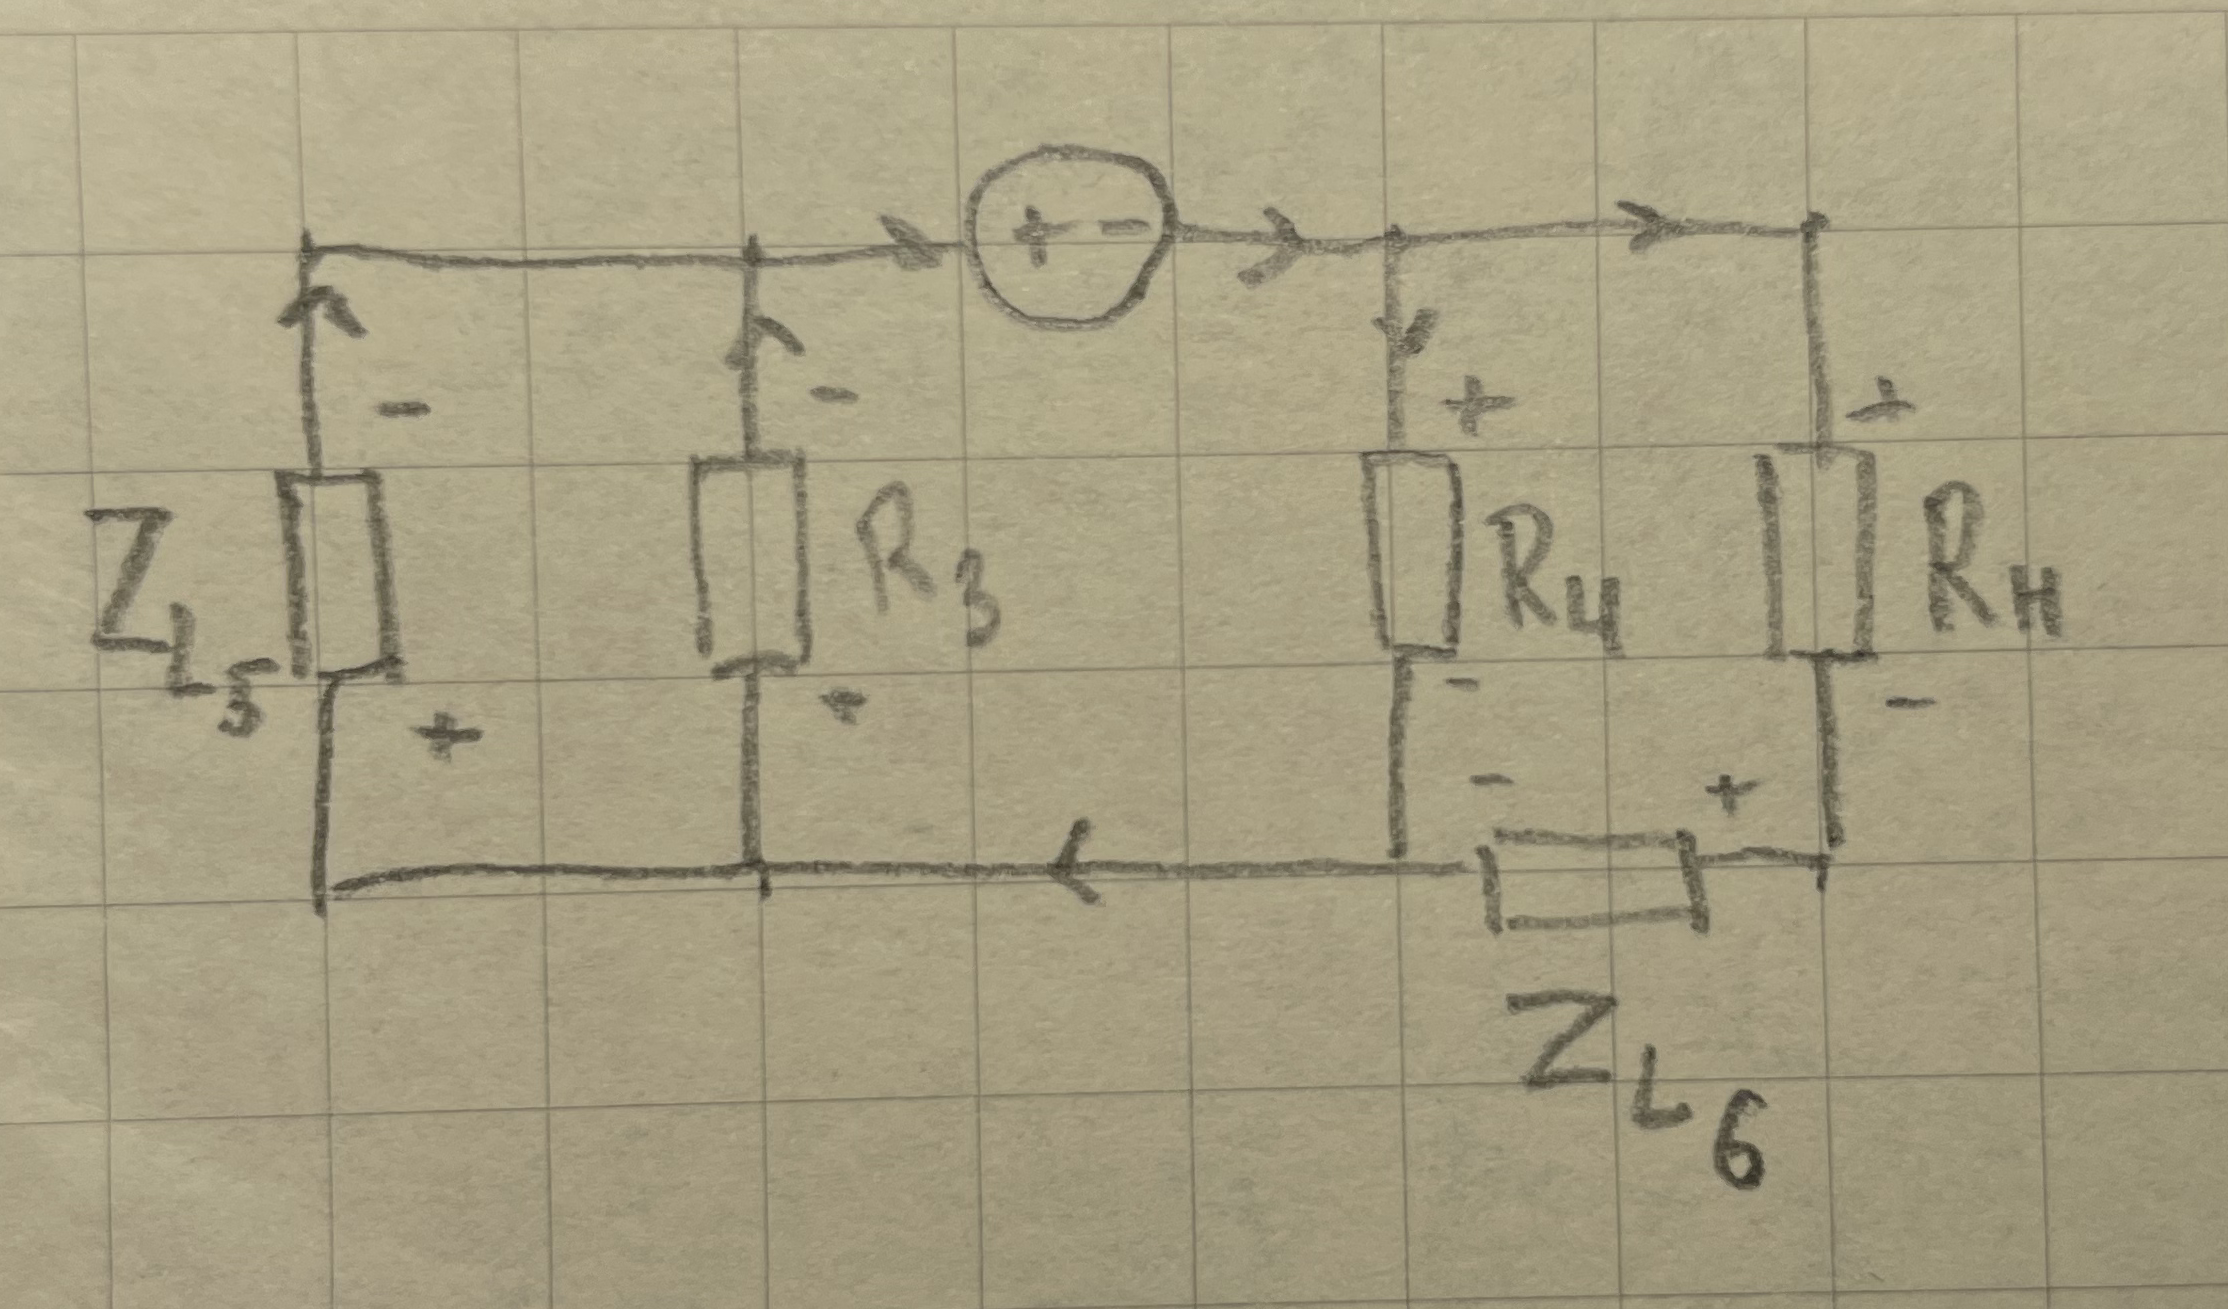
\includegraphics[width=0.7\linewidth]{photo/circ_replaced_operator}
    \caption{Операторная схема замещения}
    \label{fig:circ_replaced_operator}
\end{figure}

Найдём изображения 
реакции $ U_{R_н}(s) $ и 
воздействия $ U_1(s) $

\begin{comment}
    Комплексные сопротивления реактивных элементов:
    
    $$ Z_L = sL \; (j \omega L) $$
    
    $$ Z_С = \dfrac{1}{sC} \; (\dfrac{1}{j \omega C}) $$
\end{comment}

Для начала определим 
$ Z_{L_5}, Z_{L_6} $:

$$ Z_{L_5} = sL_5 = \dfrac{s}{2} $$

$$ Z_{L_6} = sL_6 = s \cdot 1 = s $$

$ U_{R_н} = R_н I_{R_н} $

Методом контурных токов определим 
$ I_{R_н} $ (рис. \ref{fig:mkt})

\begin{figure}[H]
    \centering
    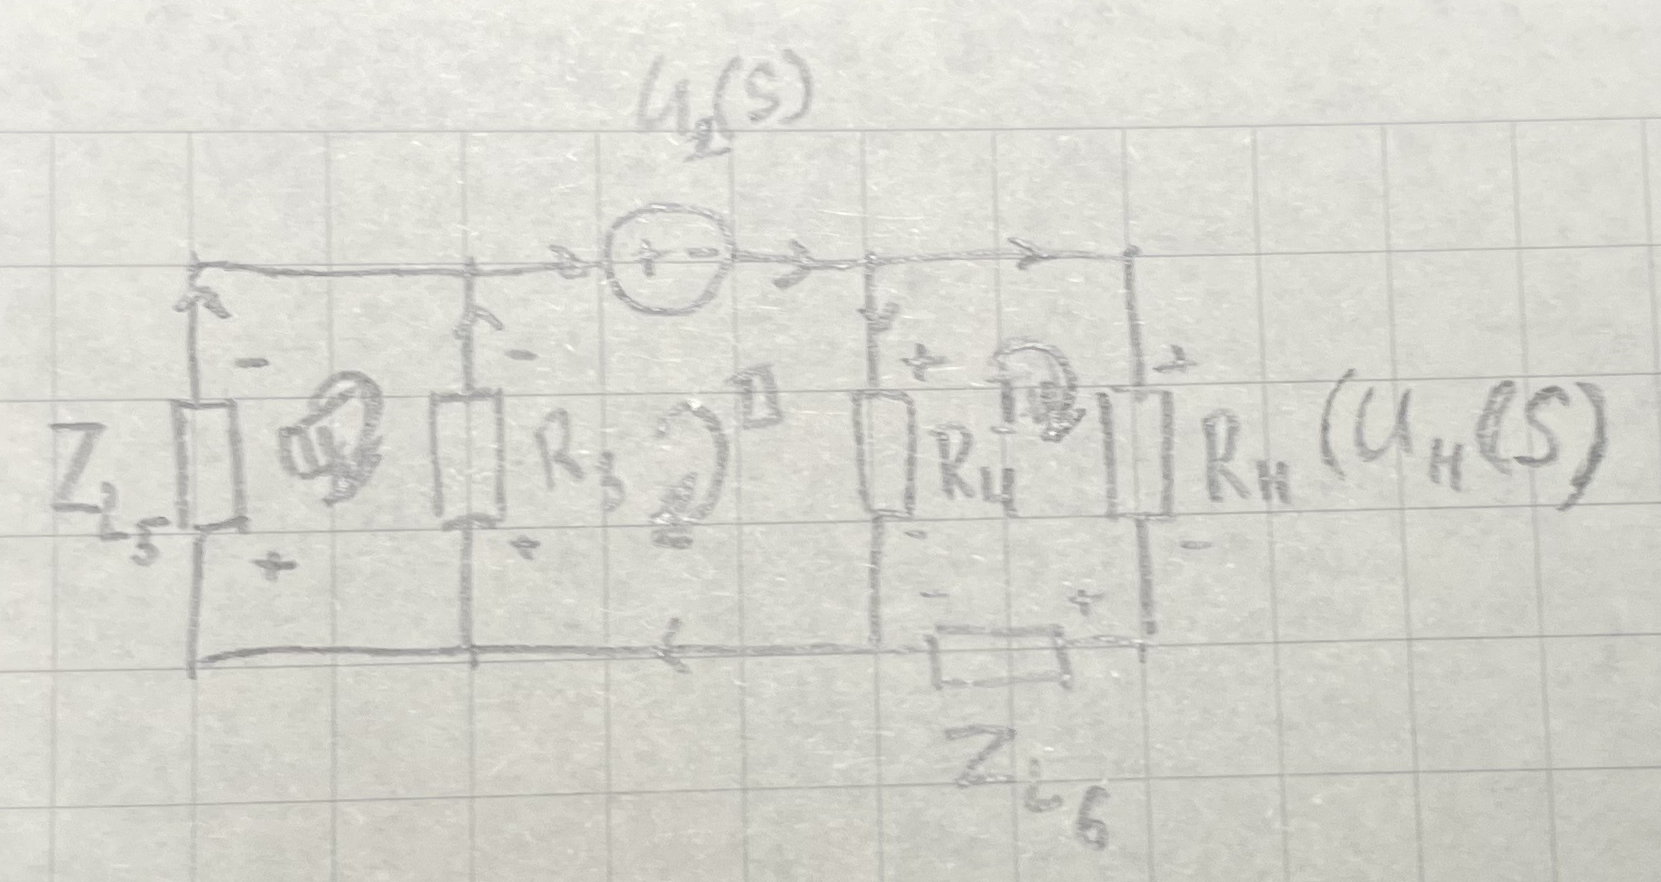
\includegraphics[width=0.7\linewidth]{photo/mkt}
    \caption{Метод контурных токов}
    \label{fig:mkt}
\end{figure}

$
\begin{bmatrix}
    R_{11} & R_{12} & R_{13}\\
    R_{21} & R_{22} & R_{23}\\
    R_{31} & R_{32} & R_{33}\\
\end{bmatrix}
\cdot
\begin{bmatrix}
    I^к_{1}\\
    I^к_{2}\\
    I^к_{3}\\
\end{bmatrix}
=
\begin{bmatrix}
    U^0_{1}\\
    U^0_{2}\\
    U^0_{3}\\
\end{bmatrix}
$\\\\

$
\begin{bmatrix}
R_4 + R_н + Z_{L_6} & -R_4 & 0\\
-R_4 & R_4 + R_3 & -R_3\\
0 & -R_3 & R_3 + Z_{L_5}\\
\end{bmatrix}
\cdot
\begin{bmatrix}
I^к_{1}\\
I^к_{2}\\
I^к_{3}\\
\end{bmatrix}
=
\begin{bmatrix}
0\\
U_1(s)\\
0\\
\end{bmatrix}
$\\\\

$
\begin{bmatrix}
3 + s & -2 & 0\\
-2 & 4 & -2\\
0 & -2 & 2 + \dfrac{s}{2}\\
\end{bmatrix}
\cdot
\begin{bmatrix}
I^к_{1}\\
I^к_{2}\\
I^к_{3}\\
\end{bmatrix}
=
\begin{bmatrix}
0\\
U_1(s)\\
0\\
\end{bmatrix}
$\\\\

$ 
\Delta_R
= 
\begin{vmatrix}
3 + s & -2 & 0\\
-2 & 4 & -2\\
0 & -2 & 2 + \dfrac{s}{2}\\
\end{vmatrix} 
=\\=
[
    (3+s) \cdot 4 \cdot (2+\dfrac{s}{2}) +
    (-2) \cdot (-2) \cdot 0 +
    (-2) \cdot (-2) \cdot 0
] -\\-
[
    0 \cdot 4 \cdot 0 +
    (-2) \cdot (-2) \cdot (3+s) +
    (-2) \cdot (-2) \cdot (2+\dfrac{s}{2})
]
=\\=
(3+s) \cdot (8+2s) - (12+4s) - (8+2s)
=\\=
2s^2 + 8s + 6s + 24 - 12 - 4s - 8 - 2s
=\\=
2s^2 + 8s + 4
$\\

Так как $ I_{R_н} = I^к_{1} $, найдём $ I^к_{1} $:

$ 
\Delta_1
= 
\begin{vmatrix}
0 & -2 & 0\\
U_1(s) & 4 & -2\\
0 & -2 & 2 + \dfrac{s}{2}\\
\end{vmatrix} 
=\\=
[
0 \cdot 4 \cdot (2+\dfrac{s}{2}) +
U_1(s) \cdot (-2) \cdot 0 +
(-2) \cdot (-2) \cdot 0
] -\\-
[
0 \cdot 4 \cdot 0 +
(-2) \cdot (-2) \cdot 0 +
U_1(s) \cdot (-2) \cdot (2+\dfrac{s}{2})
]
=\\=
4U_1(s) + sU_1(s)
=\\=
U_1(s) \cdot (4 + s)
$\\

$$ 
I_{R_н} = I^к_{1} = \dfrac{\Delta_1}{\Delta_R} = 
\dfrac{U_1(s) \cdot (4 + s)}{2s^2 + 8s + 4}
$$

\begin{equation}\label{eq:U_R_n}
U_{R_н}(s) = 
R_н \, I_{R_н} = 
\dfrac{U_1(s) \cdot (4 + s)}{2s^2 + 8s + 4}
\end{equation}

Тогда, при $ U_1(s) = 1 $, функция передачи напряжений:

\begin{equation}\label{eq:H_U_s}
H_U(s) = 
\dfrac{U_{R_н}(s)}{U_1(s)} =
\dfrac{\dfrac{4 + s}{2s^2 + 8s + 4}}{1} =
\dfrac{4 + s}{2s^2 + 8s + 4}
\end{equation}

Из (\ref{eq:H_U_s}) 
найдём $ H_U(s) $ 
при 
$ s = 0 $ и
$ s \rightarrow \infty $:

$$ H_U(0) = 1 $$

$$ H_U(\infty) = 0 $$

Проверим полученные значения 
$ H_U(0), H_U(\infty) $ по схемам замещения, 
соответствующим $ s = 0 $ 
(рис. \ref{fig:s0})
и
$ s \rightarrow \infty $ 
(рис. \ref{fig:si}). 

\begin{figure}[H]
    \centering
    \begin{subfigure}[b]{0.45\textwidth}
        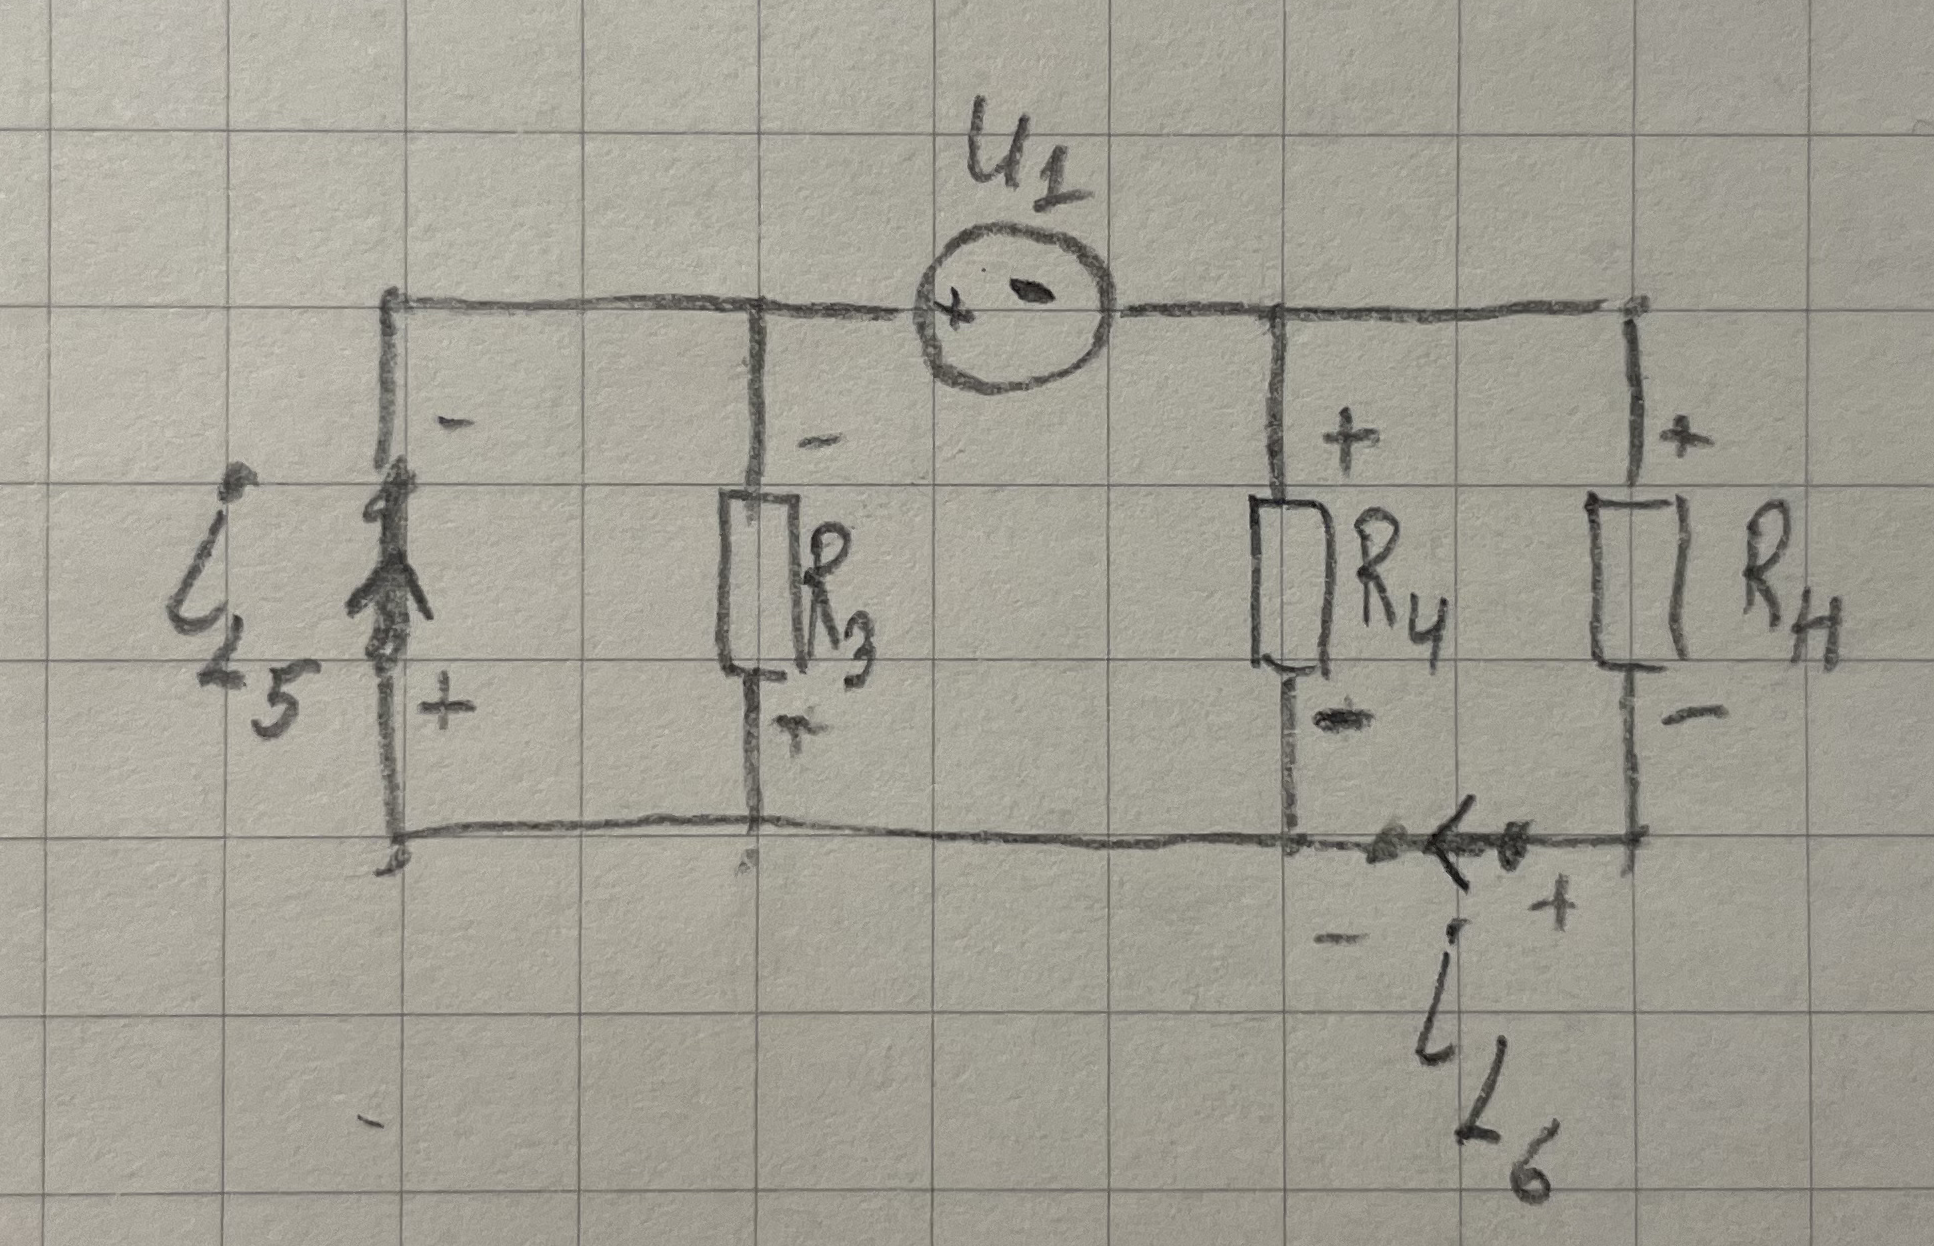
\includegraphics[width=\linewidth]{photo/circ_replaced_2}
        \caption{$ s = 0 $}
        \label{fig:s0}
    \end{subfigure}
    \hfill
    \begin{subfigure}[b]{0.45\textwidth}
        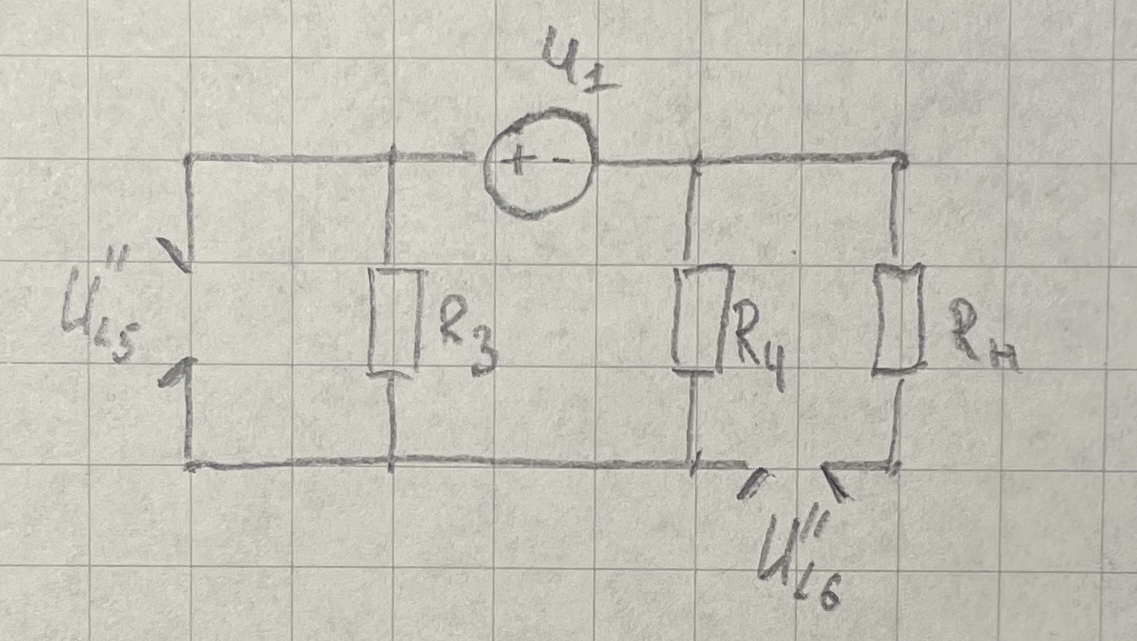
\includegraphics[width=\linewidth]{photo/circ_overlay_2}
        \caption{$ s \rightarrow \infty $ }
        \label{fig:si}
    \end{subfigure}
    \caption{Схемы замещения для проверки $ H_U(0), H_U(\infty) $}
\end{figure}

Из (\ref{eq:i_L_6_}): $ H_U(0) = 1 $

$ H_U(\infty) = 0 $

Значения совпали.

Найдем нули и полюсы функции передачи.

Нули -- корни числителя функции передачи:

$$ 4 + s = 0 \Rightarrow s = -4 $$

Полюсы -- корни занминателя функции передачи:

$ 2s^2 + 8s + 4 = 0 $

$ 
s_{1,2} = 
\dfrac{-8 \pm \sqrt{8^2 - 4 \cdot 2 \cdot 4}}{4} =
\dfrac{-8 \pm 4\sqrt{2}}{4}
$

$$
    s_{1,2} = -2 \pm \sqrt{2}
$$

Найдём переходную характеристику $ h_1(t) $

\newcommand{\lag}[1]{
    \mathcal{L}^{-1}\left[ 
        #1
    \right]
}

\newcommand{\mylim}[3][x]{
    \lim\limits_{#1 \rightarrow #2}
    \left( #3 \right)
}

$ h_1(t) = 
\lag{H_1(s)} =
\lag{\dfrac{H_U(s)}{s}} = 
\lag{\dfrac{4 + s}{s(2s^2 + 8s + 4)}} =\\\\=
\lag{
    \dfrac{A}{s} + 
    \dfrac{B}{s-s_1} + 
    \dfrac{C}{s-s_2}
}
=
\lag{
    \dfrac{A}{s} + 
    \dfrac{B}{s + 2 - \sqrt{2}} + 
    \dfrac{C}{s + 2 + \sqrt{2}}
}
$\\\\

Коэффициенты $ A, B, C $:

$ 
A = 
\mylim[s]{0}{s \dfrac{4 + s}{s\,(2s^2 + 8s + 4)}} = 
\dfrac{4}{4} = 1
$

$ 
B = 
\mylim[s]{s_1}{(s-s_1) \dfrac{4 + s}{s(s - s_1)(s - s_2)}} = 
\mylim[s]{s_1}{(s_1-s_1) \dfrac{4 + s_1}{s_1(s_1 - s_1)(s_1 - s_2)}} = 
\dfrac{4 + s_1}{s_1(s_1 - s_2)} = 
\dfrac{4 - 2 + \sqrt{2}}{(-2 + \sqrt{2})(-2 + \sqrt{2} + 2 + \sqrt{2})}
=
\dfrac{2 + \sqrt{2}}{(-2 + \sqrt{2})(2\sqrt{2})} 
=\\\\=
- \dfrac{3\sqrt{2}}{4} - 1 \approx -2.06
$

$ 
C = 
\mylim[s]{s_2}{(s-s_2) \dfrac{4 + s}{s(s - s_1)(s - s_2)}} =
\dfrac{4 + s_2}{s_2(s_2 - s_1)} =
\dfrac{4 - 2 - \sqrt{2}}{(-2 - \sqrt{2})(-2 - \sqrt{2} + 2 - \sqrt{2})}
=
\dfrac{2 - \sqrt{2}}{(-2 - \sqrt{2})(- 2\sqrt{2})}
=
\dfrac{3\sqrt{2}}{4} - 1 \approx 0.06
$

Подставим $ A, B, C, s_{1,2} $ 
в выражение переходной характеристики 
$ h_1(t) $:

$ h_1(t) = (A + B\,e^{s_1\,t} + C\,e^{s_2\,t})\delta_1(t) $

Учитывая, 
что $ s_1 \approx -0.586, s_2 \approx -3.414 $,
получим:

\begin{equation}\label{eq:h_1_t_2}
    h_1(t) = (
        1
        - 2.06\,e^{-0.586\,t} 
        + 0.06\,e^{-3.414\,t}
    )\delta_1(t)
\end{equation}

Найдём $ h_1(0), h_1(\infty) $:

$$ h_1(0) = 1 - 2.06 + 0.06 = -1 $$

$$ h_1(\infty) = 
\mylim[t]{\infty}{
    1
    - \dfrac{2.06}{e^{0.586\,t}}
    + \dfrac{0.06}{e^{3.414\,t}}
} =
1
$$

Проверим
$ h_1(0), h_1(\infty) $ по схемам замещения, 
соответствующим $ t = 0 $ ($ L = ХХ $)
(рис. \ref{fig:t0})
и
$ t \rightarrow \infty $ ($ L = КЗ $)
(рис. \ref{fig:ti}). 

\begin{figure}[H]
    \centering
    \begin{subfigure}[b]{0.45\textwidth}
        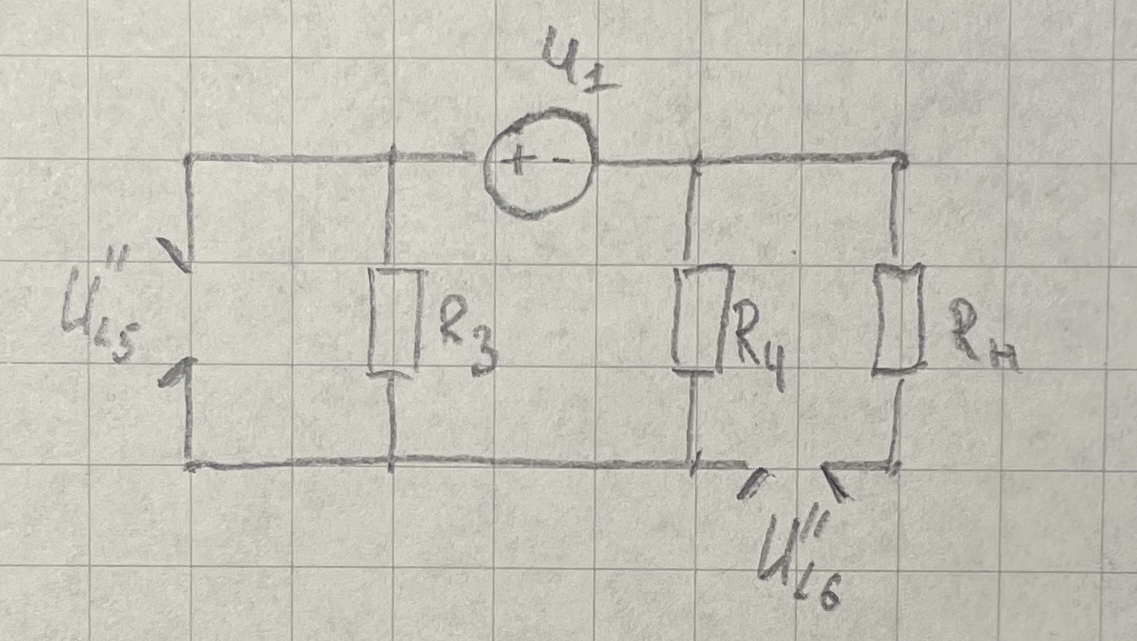
\includegraphics[width=\linewidth]{photo/circ_overlay_2}
        \caption{$ t = 0 $}
        \label{fig:t0}
    \end{subfigure}
    \hfill
    \begin{subfigure}[b]{0.45\textwidth}
        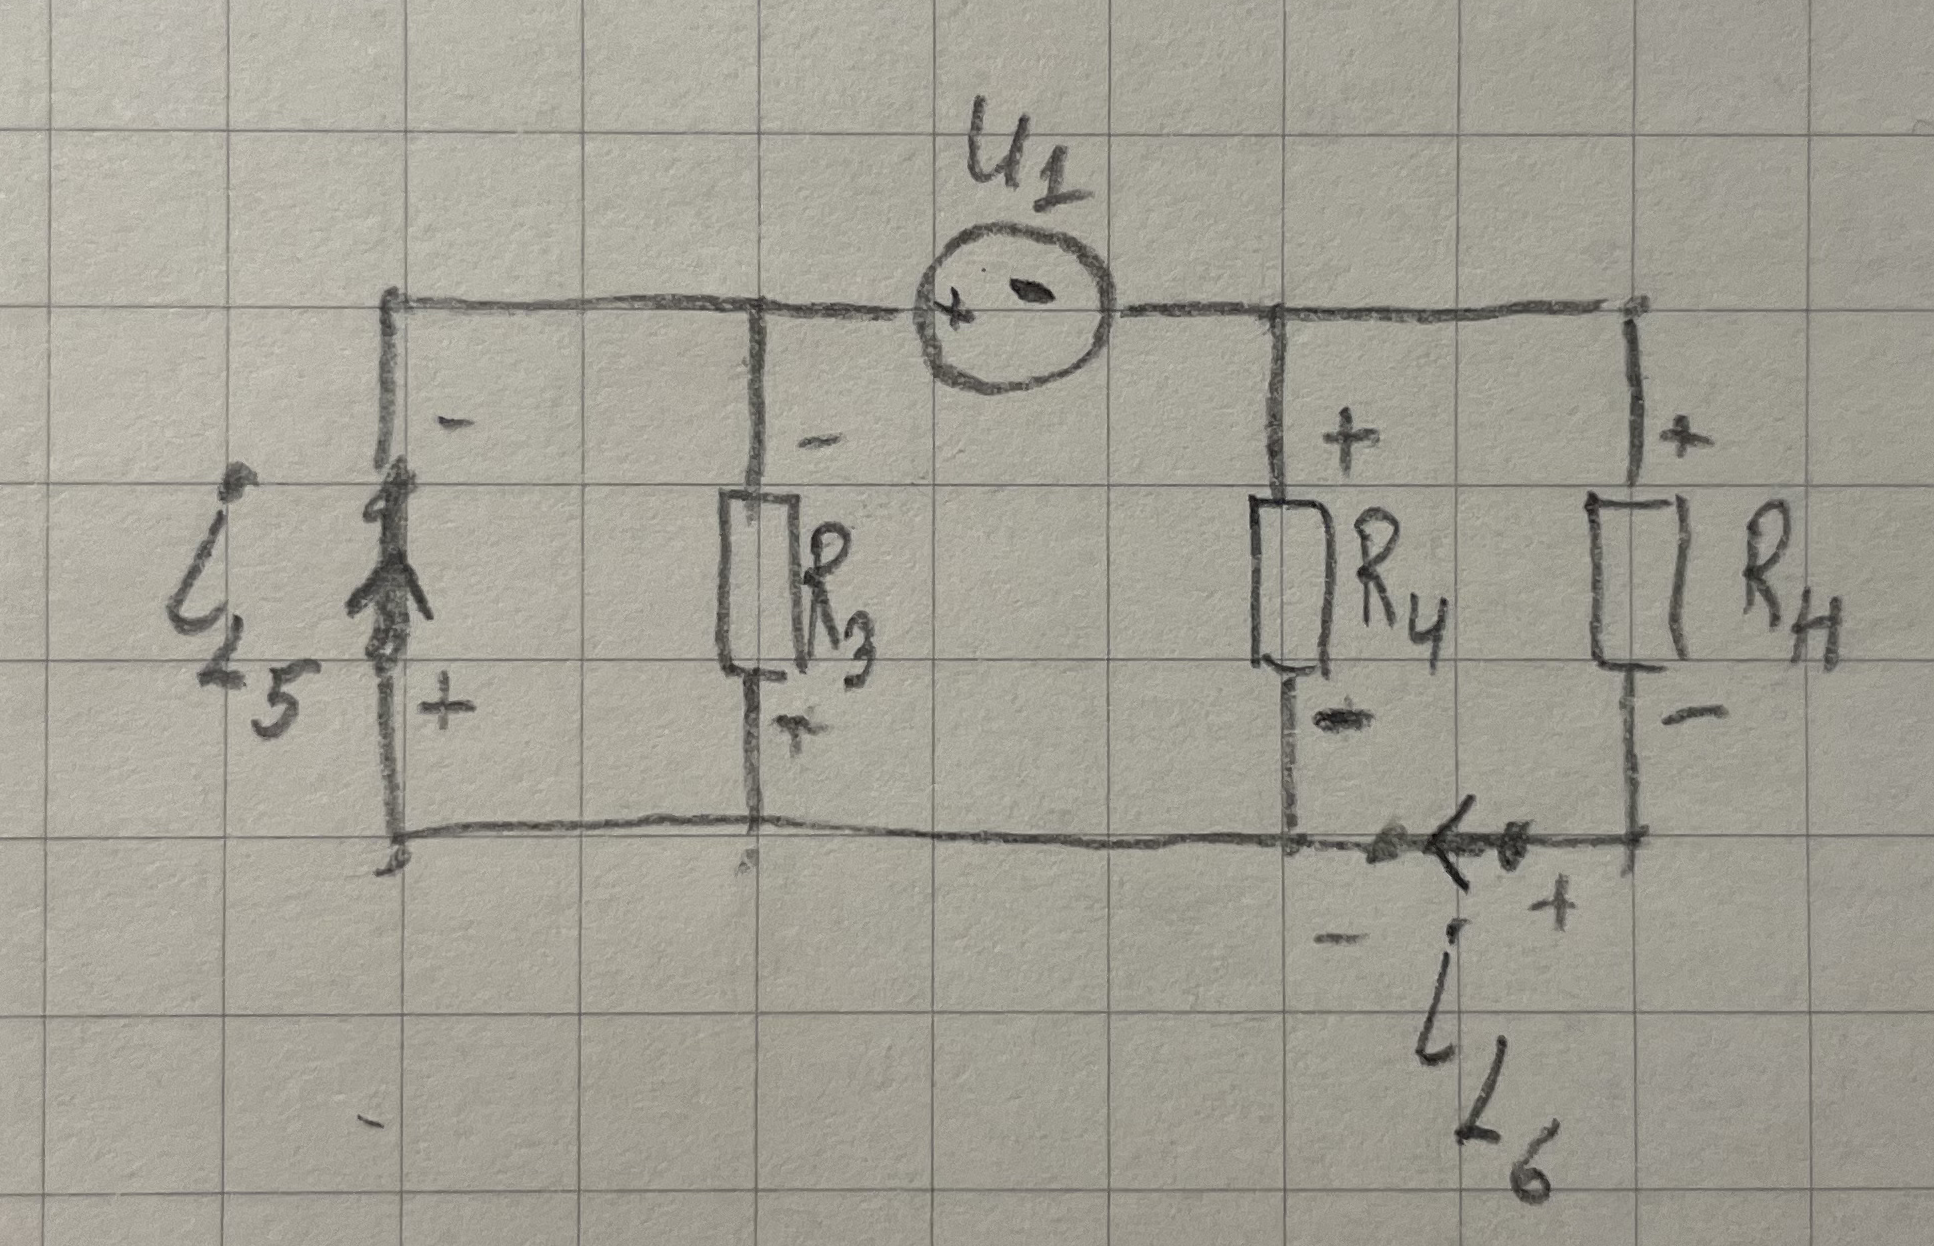
\includegraphics[width=\linewidth]{photo/circ_replaced_2}
        \caption{$ t \rightarrow \infty $ }
        \label{fig:ti}
    \end{subfigure}
    \caption{Схемы замещения для проверки $ h_1(0), h_1(\infty) $}
\end{figure}

$$ h_1(0) = U_{R_н} = -U_{R_4} = -1 $$

$$ h_1(\infty) = U_{R_н} = U_{R_4} = 1 $$

Значения, 
полученные аналитически и 
с использованием схемы замещения 
совпали.

Определим изображение по Лапласу входного одиночного импульса.

В соответствии с параметрами 
(\ref{eq:params})
и формой сигнала (рис. \ref{fig:task_plot}):

$$ 
U_1(t) = 
U_m \, \delta_1(t) - U_m \, \delta_1(t - t_и) =
7 \, \delta_1(t) - 7 \, \delta_1(t - 3)
= \left[\delta_1(t)=\dfrac{1}{s}\right] =
\dfrac{7}{s} - \dfrac{7}{s} \, e^{-3s}
$$

\begin{comment}
    Определить изображение выходного сигнала 
    и далее найти реакцию
    $ i_2(t) $ или $ u_2(t) $
    во временно́й области. 
    Построить графики входного и 
    выходного сигналов на одном рисунке.
\end{comment}

Найдем изображение выходного сигнала $ U_н(s) $
и реакцию во временной области $ u_н(t) $.

$ U_н(s) = H_U(s) \, U_1(s) = 
\dfrac{4 + s}{s\,(2s^2 + 8s + 4)}\,
\left(7 - 7 \, e^{-3s}\right)
$

$ u_н(t) =
7 \, (
1
- 2.06\,e^{-0.586\,t} 
+ 0.06\,e^{-3.414\,t} 
)
\delta_1(t) 
-\\-
7 \, (
1
- 2.06\,e^{-0.586\,(t - 3)} 
+ 0.06\,e^{-3.414\,(t - 3)} 
) \delta_1(t - 3)
$

Графики входного и выходного сигналов
представлены на рис. \ref{fig:plot_2}

\begin{figure}[H]
    \centering
    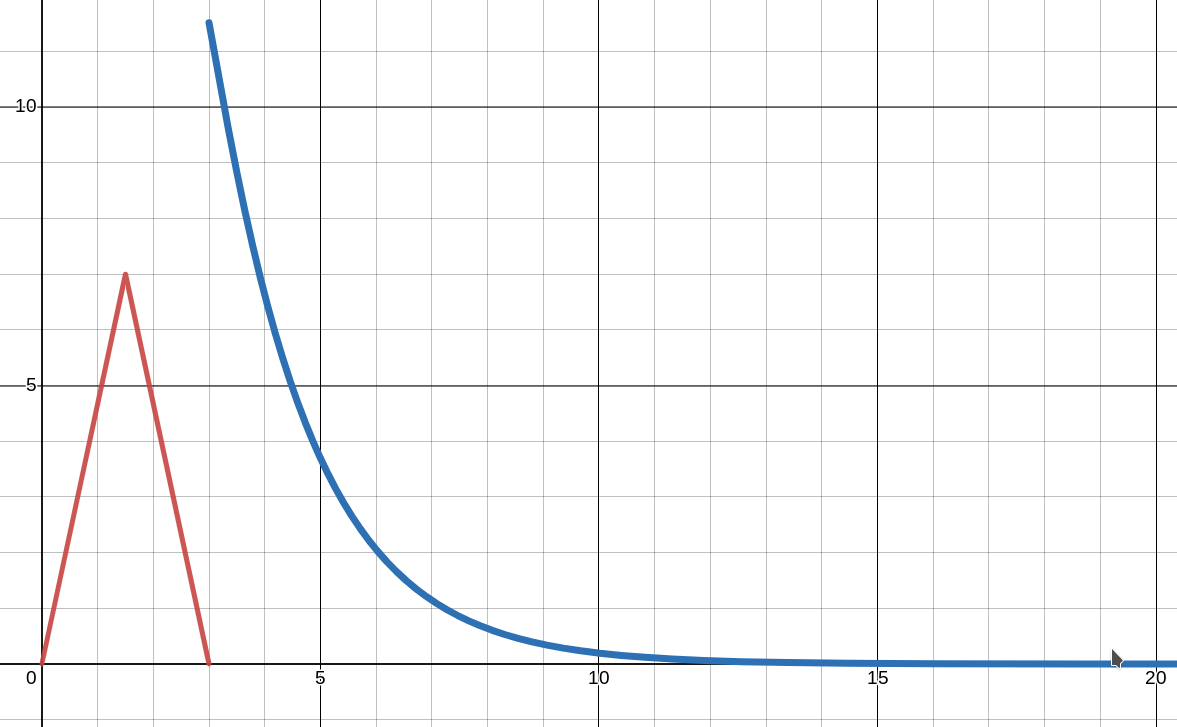
\includegraphics[width=0.7\linewidth]{photo/plot_2}
    \caption{Графики входного и выходного сигналов}
    \label{fig:plot_2}
\end{figure}


